\section{Adapting Imai and Iri to the Global Fréchet Distance}
\label{sec:global_imai_iri}

In this section, we revisit the well-known \citeauthor{computational_geometric_methods_for_polygonal_approximations_of_a_curve}~\cite{computational_geometric_methods_for_polygonal_approximations_of_a_curve} algorithm for local Fréchet polyline simplification and demonstrate how to adapt it to the global Fréchet setting. By using different graph traversals, we can obtain the algorithm from \citeauthor{on_optimal_polyline_simplification_using_the_hausdorff_and_frechet_distance}, as well as rediscover a simplification algorithm from \citeauthor{global_curve_simplification}. We modify the algorithm slightly to create a simple cubic time heuristic which achieves optimality in many cases. This heuristic only uses quadratic space in the worst case. In the best case both sapce and runtime are improved by a linear factor, i.e., it can achieve a runtime of \(\Oh(n^2)\) and a space consumption of \(\O(n)\) for sufficiently well-behaved polylines.

Throughout this section we fix \(\varepsilon > 0\) and a distance \(\delta\). Further, let \(P\) be a polyline of length \(n\). We note that some of the lemmas in this section can be seen rather trivial in the free space diagram. We have not mentioned it in this thesis because it adds a layer of abstraction which makes the algorithms less intuitive in our opinion. Furtermore, up until this section there was no need for it. An introduction to it is longer than proving the lemmas directly.

\subsection{Local Case}

We recall the algorithm in the local setting to identify where modifications are needed to adapt it to the global setting. 

The algorithm consists of two main parts: first, a shortcut graph is constructed and then, a shortest path computation yields the simplification.

The shortcut graph is a directed acyclic graph whose vertices correspond to the polyline vertices. A directed edge \((P(i), P(j))\) with \(i < j\) exists if \(\delta^F(P[i \dots j], \overline{P(i)P(j)}) \leq \varepsilon\) (i.e., \(\overline{P(i)P(j)}\) is a shortcut for the subpolyline \(P[i \dots j]\)). 

To determine whether \(\delta^F(P[i \dots j], \overline{P(i)P(j)}) \leq \varepsilon\), we use the algorithm from \citeauthor{computing_the_frechet_distance_between_two_polygonal_curves}, modified versions of which are outlined in \cref{ssec:alt_godau,ssec:implicit_frechet_decision}. Here, the simpler classical version suffices. This test requires \(\Oh(n)\) time and as there are \(\O(n^2)\) many pairs to test, constructing the shortcut graph requires \(\Oh(n^3)\) time.

Each path from \(P(0)\) to \(P(n)\) corresponds to a valid, not necessarily optimal, local simplification of the polyline by construction and it is obvious that all such simplifications are captured in the shortcut graph. Thus, computing the shorted \(P(0)-P(n)\) path in this graph yields an optimal local simplification. This can be done easily in \(\O(n^2)\).

The total runtime is determined by the cubic graph construction phase thus the total runtime is \(\Oh(n^3)\).

\subsection{The Global Shortcut Graph}
In the global case the structure of these shortcuts is more complicated, necessitating a more sophisticated approach. To confront this problem, we store for each shortcut the set of all subpolylines for which it is a valid shortcut. 

\begin{definition}
  For a shortcut \(e = \overline{P(i')P(i)}\) we say that \((t', t) \in [0, n]^2\) with \(t' \leq t\) is \emph{\(e\)-admissible} if and only if \(\delta^F(P[t' \dots t], e) \leq \varepsilon\). We denote \(\mathcal{A}_e = \set{(t', t) \mid (t', t) \textrm{ is } e\textrm{-admissible}}\) as the set of \(e\)-admissible subpolylines.
\end{definition}

The following observation might seem complicated, but it follows directly from the definitions of admissibility and Fréchet distance. It captures our intuition that global simplifications are constructed of only admissible subpolylines.

\begin{observation}
	Let \(Q=\angl{P(u_0), \dots, P(u_q)}\) be a (not nessarily optimal) global simplification of \(P\) which means there are parameterizations increasing, continuous \(f, g\) with \(f([0, 1]) = [0, n]\) and \(g([0,1]) = [0, q]\) with \(\delta(P(f(\alpha)), Q(g(\alpha))) \leq \varepsilon\) for all \(\alpha \in [0, 1]\).

	Then, for \(i \in \set{1, \dots, q}\) and \(x \leq y \in [0, 1]\) such that \(g(x) = i - 1\) and \(g(y) = i\) it holds that 
	\[\delta^F(P[f(x) \dots f(y)], \overline{P(g(x)), P(g(y))}) \leq \varepsilon.\]
	This means \((f(x), f(y))\) is \(e\)-admissible for \(e = \overline{P(g(x), P(g(y)))} = \overline{Q(i-1), Q(i)}\).
\end{observation}

Next, we explore the set of admissible subpolylines \(\mathcal{A}_e\) with the goal of establishing an efficient representation.

\begin{lemma}\label{lem:admissible_are_intervals}
	Let \(e = \overline{P(i')P(i)}\).
  \begin{enumerate}
		\item Let \((r, t)\in \mathcal{A}_e\) and \(r \leq t' \leq t\) with \(\delta(P(t'), P(i')) \leq \varepsilon\). Then \((t', t) \in \mathcal{A}_e\).
		\item Let \((t', r)\in \mathcal{A}_e\) and \(t' \leq t \leq r\) with \(\delta(P(t), P(i)) \leq \varepsilon\). Then \((t', t) \in \mathcal{A}_e\).
  \end{enumerate}
\end{lemma}

\begin{proof}
	We show the first statement. The second one is analogous. We create suitable parameterizations \(f\) and \(g\) to show \(\delta^F(P[t' \dots t], e) \leq \varepsilon\). As \((r,t)\) is \(e\)-admissible, there are functions increasing, bijective parameterizations \(f':[0,1] \to [r \dots t]\) and \(g':[0,1] \to [0,1]\) (here we shift the range of \(f'\) to be consistent with \(P\) and not the subpolyline \(P[r \dots t]\)).

	Since \(f'\) is surjective onto \([r, t]\) and \(t' \in [r, t]\), there is \(x \in [0, 1]\) with \(f'(x) = t'\). This means that \(\delta(P(t'), e(g'(x))) \leq \varepsilon\). By the convexity property in \cref{lem:distance_properties}, \(\delta(P(t'), e(\lambda)) \leq \varepsilon\) for all \(\lambda \in [0, g'(x)]\). With this, we construct the parameterizations \(f\) and \(g\) such that \(f\) is the zero function until \(g\) assumes the value \(g'(x)\). After this point both functions are identical to \(f'\) and \(g'\) respectively (up to a shift in the range).
\end{proof}

\begin{definition}
	For sets \(A\) and \(B\) we define \(A \times_{\leq} B\) to be 
		\[A \times_{\leq} B = \set{(a, b) \in A \times B \mid a \leq b}.\]
\end{definition}

Using \cref{lem:admissible_are_intervals}, we define an efficient representation of \(\mathcal{A}_e\).
\begin{lemma}\label{lem:admissible-rep-1}
	Let \(e = \overline{P(i')P(i)}\) be a line segment. Denote \(\mathcal{I} = \set{t \in [0,n] \mid \delta(P(i'), P(t)) \leq \varepsilon}\) and \(\mathcal{J} = \set{t \in [0,n] \mid \delta(P(i), P(t)) \leq \varepsilon}\). There exist \(k \leq n\) and families of closed intervals \(I_1 \leq \cdots \leq I_k\) and closed intervals \(J_1 \leq \cdots \leq J_k\) such that 
	\[\mathcal{A}_e = \parenth{\mathcal{I} \times_\leq \mathcal{J}} \cap \bigcup_{j=1}^k I_j \times J_j.\]

	Here, the ordering on the intervals is defined by their lower bounds or equivalently by their upper bounds. It is further possible to achieve that the family \(I_j\) is pairwise disjoint or that the family \(J_j\) is pairwise disjoint (but not necessarily both).
\end{lemma}

\begin{proof}
	The lemma is trivial if \(\mathcal{A}_e\) is empty. Suppose it is not empty. It holds by definition that \(\mathcal{A}_e \subseteq \mathcal{I} \times_\leq \mathcal{J}\). 

	For any \(e\)-admissible subypolyine \((t', t)\) there exist closed maximal intervals \(I\) and \(J\) with \(t' \in I\), \(t' \in J\), and \(I \subseteq \mathcal{I}\) and \(J \subseteq \mathcal{J}\) by the distance constraints on the endpoints by the definition of the Fréchet distance. 

	We show that \(I \times_\leq J \subseteq \mathcal{A}_e\): pick any \(s' \leq s\) with \(s' \in I\) and \(s \in J\). If \(s' \leq t'\) then \(\delta^F(P[s' \dots t'], P[y \dots y]) \leq \varepsilon\) for any \(y \in J\) by construction of \(I\) and \(J\), and thus, we can extend any admissible \(t', y\) subpolyline to an admissible \((s', y)\). Similarly, if \(s \geq t\), for any \(x \in I\), we can extend admissible \((x, t)\) subpolylines to admissible \((x, s)\) subpolylines. Therefore, we can assume \(s' \geq t'\) and \(t \leq s\). Under these conditions, it follows that \((s', s)\) is admissible by using \cref{lem:admissible_are_intervals}.

	We now have seen that admissibility is a property shared by pairs of intervals, not only points. Thus, we will say \((I, J)\) is admissible if all point pairs \((t', t)\) with \(t' \leq t\) in \(I \times J\) are admissible.


	This shows that \(\mathcal{A}_e\) has almost such a structure. We need to show that \(k \leq n\) many interval pairs suffice. For this, we merge intervals: Let \(I < I'\) disjoint and \(J\) be closed intervals that we have already selected for the construction. Furthermore, assume that \((I, J)\) and \((I', J)\) are admissible. By \cref{lem:admissible_are_intervals}, for any point \(x \in [\min I, \max I'] \cap \mathcal{I}\) any \(y \in J\) with \(x \leq y\) must form an admissibily subpolyline \((x, y)\). Thus we merge all such intervals \(I'\) and \(I\) to form an interval of intervals per interval \(J\). This does not introduce no inadmissible subpolylines, as we already filter by \(\mathcal{I} \times_\leq \mathcal{J}\). As each interval \(J\) has a unique range of intervals \(I\), the \(J_j\) are disjoint. By merging the \(J\) per \(I\) instead, we can achieve disjointness of \(I_j\).

	The total number of interval pairs is bounded by the number of possible closed intervals that make up \(\mathcal{I}\) and \(\mathcal{J}\). There can be at most one closed interval per line segment of the polyline, thus \(k \leq n\), concluding the proof.
\end{proof}


\begin{definition}[Global Shortcut Graph]
	For a polyline \(P = \angl{v_0, \dots, v_n}\) and \(\varepsilon > 0\) we define the global shortcut graph as the directed acyclic graph \(G = (V, E)\) with \(V = \set{v_0, \dots, v_n}\) and \(E = \set{(v_i, v_j) \mid i < j, e = \overline{v_iv_j}, \mathcal{A}_e \neq \emptyset}\).

	We define a labelling function on the edges 
	\[S(e) = ((I_1, J_1), (I_2, J_2), \dots, (I_k, J_k)),\]
	where the intervals \(I_i, J_i\) are taken from the proof of \cref{lem:admissible-rep-1}. We extend this labelling on the vertices by \(S(v) = (I_1 < \cdots < I_k)\), which are the intervals that make up \(\mathcal{I}\) from the lemma.

	We refer to intervals \(I \in S(v)\) as \emph{solution intervals} as they are defined by solving equations. A pair \((I, J) \in S(e)\) will be referred to as a \emph{(interval) mapping} as the describe how to map points \(I\) to points in \(J\) using the shortcut \(e\).
\end{definition}

Let us briefly analyze the space consumption of the global shortcut graph: for each line segment, we may need to store up to \(n\) mappings, which in total requires cubic space. There are at most \(n\) solution intervals in \(\mathcal{I}\) per point, thus requiring total quadratic space. The total information of the global shortcut graph requires \(\O(n^3)\) space. This, however is only the worst case. Since solution intervals can span multiple line segments which we merge into a single interval to obtain fewer intervals. For further analysis, we denote \(\mathcal{E}\) the total number of mappings in the edges and \(\mathcal{V}\) for the number of solution intervals for the vertices. The total space thus is \(\O(n^2 + \mathcal{E})\).

We finally consider the runtime of constructing the global shortcut graph. For the point \(u\), the solution intervals \(S(u)\) can be determined by solving the necessary equation for each line segment of \(P\) and potentially merging ones that span multiple line segments. This takes runtime \(\Oh(n)\) per point and thus in total \(\Oh(n^2)\). 

To determine the mappings in \(S(e)\) for the line segment \(e = \overline{P(i')P(i)}\), we use a modified version of \citeauthor{polyline_simplification_has_cubic_complexity_bringmannetal}'s cell reachability algorithm that we have outlined in \cref{ssec:cell_reachability}.

\subsection{Modified Cell Reachability}
We describe how to modify the cell reachability problem to construct the interval mappings in \(S(e)\). We are given the ordered lists of solution intervals \(S(i')\) and \(S(i)\) and want to find the mappings between them. 

The setting is rather similar to \cref{ssec:cell_reachability} with few differences. First, there are no entry- or exit-costs, we only track admissibility. Second, the result is an interval \(J_j\) for each admissible interval \(I_j\). The passages between cells are the solution intervals of \(e\) and the respective vertex. For an example instance refer to \cref{fig:ex_cr_globalii}.

Only few modifications are needed: For each passge, we remove all queue entries at the front with a value below the lower bower bound of the passage and reinsert them with them as a single entry whose value is the lower bound. Each entry is now associated with an interval of indices which correspond to the intervals in \(S(i')\). When merging, we update the upper bound of the indices interval. If an interval in \(S(i')\) starts before the cell passage, it must be accounted for during the merging step.

Then, we remove all entries that lie above the upper end of the passage. Each of them contains an indices interval that represent  the intervals for which the last seen \(S(j')\) interval is the upper end. For all of these intervals we update their upper bound.

The intervals in \(S(i)\) can be ignored, if we are only interested to compute maximal intervals \(J_j\) for each \(I_j\). We can consider them to only store discrete intervals that represent the intervals in \(S(i)\) that are to be used.

\begin{figure}[htb]
  \centering
  \includegraphics[scale=1, width=0.9\linewidth]{./tikz-fig/ex_cr_globalii.pdf}
	\caption{Cell reachability example for computing \(S(\overline{P(0)P(1)})\). Here, \(S(0) = ([0, 0.5], [2.5, 2.5]), [3.59, 4.36]\) are marked in blue, and \(S(1) = ([0.5, 1.70], [2.5, 2.5], [4.64, 5])\) are marked in red. The one point interval \([2.5,2.5]\) is shared by both and is marked in purple. It is not a vertex of the polyline. We can see that \(S(\overline{P(0)P(1)}) = (([0,0.5], [0.5,5]), ([2.5,2.5],[2.5,5]), ([3.59,4.36],[4.64,5]))\).}
  \label{fig:ex_cr_globalii}
\end{figure}

A small optimization that can be applied is to skip cells when the queue becomes empty and resume at the next \(S(i')\) interval. Using this, the total runtime per line shortcut is proportional to the total length of the intervals which extends to the construction of the shortcut graph. Furthermore, we can actually skip all computations when adding an interval up to the end of the interval if it is the only element in the queue (and thus especially for the first interval). This is because the lower bound for the interval is zero throughout the interval.

\subsection{Simplification Construction}

To construct the simplifications from the graph, we iterate through it using the admissible subpolylines. Any simplification is a sequence of \(e_i\)-admissible subpolylines where the sequence of edges \(e_i\) form a 0-n-path and the endpoints of two consecutive subpolylines match.

Unlike the local case, it does not suffice to find a shortest path, thus we have to consider more wisely how to iterate through the graph. Interestingly, we can derive the algorithm from \citeauthor{on_optimal_polyline_simplification_using_the_hausdorff_and_frechet_distance} using suitable graph traversels: we start with \(S(0)\) as the starting interval and traverse the graph. In the subsequent traversals we repeat this procedure but start with the computed intervals from the last step. We stop once an interval is found that contains the endpoint of the polyline.

From this, we can see why the \citeauthor{on_optimal_polyline_simplification_using_the_hausdorff_and_frechet_distance} algorithm has poor runtime: we iterate through the whole graph multiple times. Furthermore, their algorithm does not precompute the global shortcut graph but computes everything once it is used which also means that the same computations are performed multiple times. Using our precomputed graph the runtime can be reanalyzed as follows: let the simplification size be \(k\), then the total runtime is \(\Oh(n^3 + kf(n))\) where \(f(n)\) is the runtime per iteration and \(\Oh(n^3)\) the runtime to construct the graph.

Let us analyze how many intervals there can be at most that need to be tracked: each interval is paired with an vertex from the polyline where the vertex represents the last point of the partial simplification (i.e., the point form which we start the next shortcut) and the interval is the end of the subpolyline. As seen previous, there can be at most one interval per line segment but as it can be paired with different points, there can be in total \(\O(n^2)\) many intervals per iteration to track. For each interval we must iterate over all possible shortcuts that start from its associated end vertex to compute the next interval and verex pairs. There are at most \(\O(n^2)\) many possibilities to iterate through, resulting in \(\O(n^4)\) runtime per traversal and thus in total \(\Oh(kn^4)\) runtime. This improves upon the standard algorithm by \(\O(n)\). Furthermore, this version of the algorithm benefits more from the well-behavedness of the input by having fewer intervals to track.

To obtain a better runtime, we traverse the graph only once. The most obvious iteration order is through the graph vertices which corresponds to the same order in the algorithm by \citeauthor{polyline_simplification_has_cubic_complexity_bringmannetal} however the resulting algorithm is different. We track all subpolylines that have a partial simplification that end in the currently tracked vertex. In the local case we iterate for each vertex over all previous vertices, test if there is a shortcut to the current vertex and if so extend the partial simplification and use the minimal found partial simplification. In the global case, we can also minimize over all previously computed values and extend the previously found partial simplifcations to one ending in the current vertex, however there is more data to track.

First, we consider how much data needs to be tracked per vertex in the iterations. Each subpolyline is an interval on the polyline. Per line segment on the polyline at most \(n\) many subpolylines can start because we track only minimal subpolylines. Each subpolyline is associated with the length of the partial simplification up to this point so if we have two subpolylines starting on the same line segment with the same length, we only need to track the one with the earlier start. Thus in total only \(\O(n^2)\) subpolylines can exist.

To propagate these subpolylines for the vertex \(i\), we iterate over all \(j < i\) and use \(S(\overline{P(j)P(i)})\). We iterate over all values in \(S(j)\) to find the previous subpolylines and iterate over all mappings in \(S(\overline{P(j)P(i)})\). We iterate in simultaneously over both of them to determine all possible subpolylines that use \(j\). As \(S(j)\) has \(\O(n^2)\) many subpolylines, the mapping also requires \(\O(n^2)\) time. As this needs to be done for all \(j < i\) we get cubic runtime for the mapping. We finally need to merge all the computed subpolylines which can be done while mapping by using \(n\) linked lists, one for each line segment. Each of those lists has size \(\O(n)\) and we can store pointers to the list elements in an array to find in constant time the position of a subpolyline with a given simplification size. For this, we observe the on each line segment, the subpolylines are ordered by the start of the subpolyline in ascending order and the size of of the simplification in descending order (if a subpolyline start before another one and requires a shorter simplification, the other one can be removed).

This results in a \(\Oh(n^4)\) algorithm as there are \(\O(n)\) propagation steps which takes \(\O(n^3)\) time. Using insights from \citeauthor{polyline_simplification_has_cubic_complexity_bringmannetal}, \citeauthor{global_curve_simplification} further improved the runtime to \(\Oh(n^3)\). Both algorithms works essentially the same way but with a different order of computation.

\subsection{Cubic Runtime Heuristic}
As the cubic runtime variant of this algorithm is very similar to the \citeauthor{polyline_simplification_has_cubic_complexity_bringmannetal} algorith, we instead establish a simpler heuristic which results in smaller simplifications than local simplifications and achieves optimal results in many cases.

The main problems of the cubic variants are their rigid structure that force a cubic number of computations which seem to be resistant to further optimizations. The current \(\Oh(n^4)\) algorithm can adapt to the input to achieve up to near quadratic runtime and space in the best case.

To achieve worst case \(\Oh(n^3)\) time and quadratic space with possibly quadratic runtime for well-behaved polylines, we introduce a new heuristic based on the case distinction that both of the cubic runtime algorithms make. In \citeauthor{polyline_simplification_has_cubic_complexity_bringmannetal}'s algorithm, we distinguish the case carrying over the earliest reachable point on the same line segment or setting the earliest reachable point to the start of the solution interval when comparing different line segments. The first case is computed using a simple minimum computation while the second one requires the cell reachability procedure.

Even though the first of the two cases is simpler to compute, it causes the most problems: It is the reason why we need cubic space as we need to track linearly many points per line segment and vertex; the second case only requires one datum per line segment. Additionally, intuitively this case is less likely to affect the simplification. In this case we have multiple consective shortcuts that make little progress on the polyline which is in opposition to the goal of achieving as few shortcuts as possible. Furthermore, interval mappings that allow make this case necessary have a restrictive nature. 

To formlize our approach, we split mappings into three categories:
\begin{definition}
	Let \(m = ([a, b], [c, d])\) be a mapping in the global shortcut graph. We call \(m\)
	\begin{itemize}
		\item \emph{positive} if \(b \leq c\),
		\item \emph{neutral} if \(a \leq c \leq b\),
		\item \emph{negative} if \(c < a\).
	\end{itemize}

	We call global shortcut graph positive if it has no negative mappings. A polyline is called \(\varepsilon\)-positive its global shortcut graph is positive. If \(\varepsilon\) is clear from context we will omit it.
\end{definition}

\begin{theorem}
	Let \(\varepsilon > 0\) and \(P\) be positive polyline. Then \(\delta^F(P, \varepsilon)\) can be computed in \(\Oh(n^3)\) with quadratic space.
\end{theorem}

\begin{proof}
	It is obvious that per interval and vertex only at most one reachable subpolyline must be stored when simplifying a positive polyline by reanalyzing our reasoning for the \(\Oh(n^4)\) algorithm. Thus an array of size \(\O(\mathcal{V}) \subseteq \O(n^2)\) suffices where we store for each vertex \(u\) and interval \(I \in S(u)\) the shortest partial simplification ending in \(u\) that reaches \(I\). For this only the preceding vertex and the size of the partial simplification need to be stored. With this, a graph traversal more similar to the algorithm from \citeauthor{computational_geometric_methods_for_polygonal_approximations_of_a_curve} can be applied. For each vertex \(v\), we iterate over all \(u < v\) and the reachable subpolylines in all reachable \(S(v)\) and their mappings \(S(\overline{uv})\). As all of these list are ordered and at most one mapping is applicable to any interval in \(S(v)\), the propagation onto \(u\) takes constant time per interval. For each vertex there are at most linearly many mappings and intervals to consider so by using the order, a merge-like procedure requires only linear time per \(v\) and thus quadratic time per \(u\). In total cubic runtime is achieved. 

	To reduce space to quadratic, we observe that we do not need to precompute the mappings as the mappings in \(S(\overline{uv})\) are used all at once when propagating reachability from \(u\) to \(v\) and thus, we can defer the computation to the propagation instead of storing them global. At any time only at most linearly many mappings are stored.
\end{proof}

As not every polyline is positive for a given \(\varepsilon\), we introduce a new heuristic simplification by transforming the global shortcut graph of the polyline into an positive one. This does not always yield optimal simplifications but the simplifications are never worse than local ones.

The first step is to split the unique interval \(I = [a, b] \in S(u)\) with \(u \in I\) into two intervals \([a, u]\) and \([u, b]\). The second and final step consists of narrowing the intervals in \(S(u)\) for all \(u\) and removing mappings in the following way. For any mapping negative \(([a,b], [c,d]) \in S(\overline{uv})\) with we either 
\begin{enumerate}
	\item update the first interval \([c, x] \in S(u)\) to \([a, x]\) if \(a \leq x\),
	\item If \(a > x\), we remove the interval \([c, x]\) from the mapping. If there are further intervals in the range of the mapping we repeat this process with the next interval until the first case occurs or no intervals remain in the range. In the latter case, we remove the mapping completely.
\end{enumerate}

After this process, the global shortcut graph is positive as we have modifed or removed all negative mappings. We now show that using this modified shortcut graph always yields a solution that is not worse than a local simplification. For this it suffices to show that all local shortcuts are still included. Take a local shortcut \(\overline{uv}\), which means that \(\delta^F(P[u \dots v], \overline{uv}) \leq \varepsilon)\). This means that \((u, v)\) is \(\overline{uv}\)-admissible and thus there is a mapping \((I, J) \in S(\overline{uv})\) with \(u \in I\) and \(v \in J\). Since we have split the solution intervals containing \(u\) in \(S(u)\), no intervals are removed in the process, and the intervals are only shrunk from the left, there is still an interval \([a, u]\) in \(S(u)\) and similarly for \(v\). The mapping that contains the local shortcut can not be removed by this process because \(u < v\). Thus all local shortcuts are still contained in the graph. Of course, a consequence of this is that this process can never remove too many mappings and thus will always find a solution.

To achieve quadratic space, we still do not need to precompute the whole global shortcut graph. When computing the reachable subpolylines for \(v\) the mappings in \(S(\overline{uv})\) only affect the solution intervals in \(S(v)\). It suffices to shrink the intervals as the mappings are computed and store the reachable subpolylines as an interval of indices (because the indices of the solution intervals do not change unlike their left bounds).

This heuristic can also be made into a simple optimal algorithm: for each negative mapping \(([a,b], [c,d]) \in S(\overline{P(i')P(i)})\) we split the interval \([c, d] \in (S(i))\) into two intervals \([c, a]\) and \([a, d]\). This basically transforms the heuristic back into the \(\Oh(n^4)\) algorithm as the amount of intervals can be quadratic per vertex. Using other interval-splitting and mapping-update strategies might yield better results than the outlined heuristic at the potential cost of runtime.

\subsection{Analysis of the Heuristic}
We have shown that our heuristic is never worse than a local simplification. Now, we analyze polylines on which the heuristic performs well and ones where it performes poorly.

The examples \cref{fig:local-global-bigdiff,fig:local-global-mostdiff} which have a high difference between the local and global simplifications can be solved optimally using our heuristic as both polylines are \(\varepsilon\)-positive using the given \(\varepsilon\). For further investigations into optimality criteria for the heuristic we differentiate polylines into two categories.

\begin{definition}
  Let \(P\) be a polyline and \(\varepsilon > 0\). We call \(P\)
	\begin{itemize}
		\item \(\varepsilon\)-\emph{neutral} if the result from the heuristic is optimal and 
		\item \(\varepsilon\)-\emph{negative} if the result from the heuristic is non-optimal.
	\end{itemize}
\end{definition}

Naturally, every positive polyline is also neutral and any the shortcut graph of a negative polyline contains at least one negative mapping. 

Let us present a few simple criteria for neutral polyines.
\begin{lemma}
  Let \(P\) be a polyline, \(\varepsilon > 0\) and \(G\) be the global shortcut graph of \(P\) using \(\varepsilon\). \(P\) is \(\varepsilon\)-neutral if any of these following conditions hold.
	\begin{enumerate}
		\item \(P\) is \(\varepsilon\)-positive.
		\item The local and global simplifications of \(P\) coincide.
		\item \(\varepsilon\) is at least as large as the distance between any pair of vertices of \(P\).
		\item \(S(i)\) contains exactly one solution interval and this unique interval contains only one polyline vertex (which must be \(i\)).
		\item \(\max \set{a \mid [a, b] \in S(i')} \leq \min \set{a \mid [a, b] \in S(i)}\) for all \(i' < i\).
	\end{enumerate}
\end{lemma}

\begin{proof}
	\begin{enumerate}
	  \item Already shown previously.
		\item The heuristic can never be smaller as the global simplification but it also cannot be larger than a local simplification.
		\item This implies both previous criteria. Each vertex contains exactly one interval \([0, n]\), i.e., each interval spans the whole polyline. As all intervals are the same there can be no negative mappings. Furthermore, this also implies that both the loval and global simplification only contain the start and end vertex.
		\item The interval in \(S(i)\) starts either on the line segment before the vertex \(i\) or the exactly on the vertex \(i\) (e.g., for \(i=0\)). Mapping the starts of the intervals onto the real numbers yields a monotone sequence. As shortcuts can only proceed to higher indexed vertices, the range interval must start after the domain interval and is thus neutral or positive. Thus, the polyline is positive.
		\item Follows directly from the proof for the last criterion.
	\end{enumerate}
\end{proof}

We present a negative polyline in \cref{fig:gii_diff_2}. The global simplification requires only four points while the heuristic needs 6. In the sequence of mappings in the global simplification there are no negative mappings, however, the heuristic stil cannot find it as the interval for the second vertex of the simplfication is shrunk because of other negative mappings. 

\begin{figure}[htb]
  \centering
  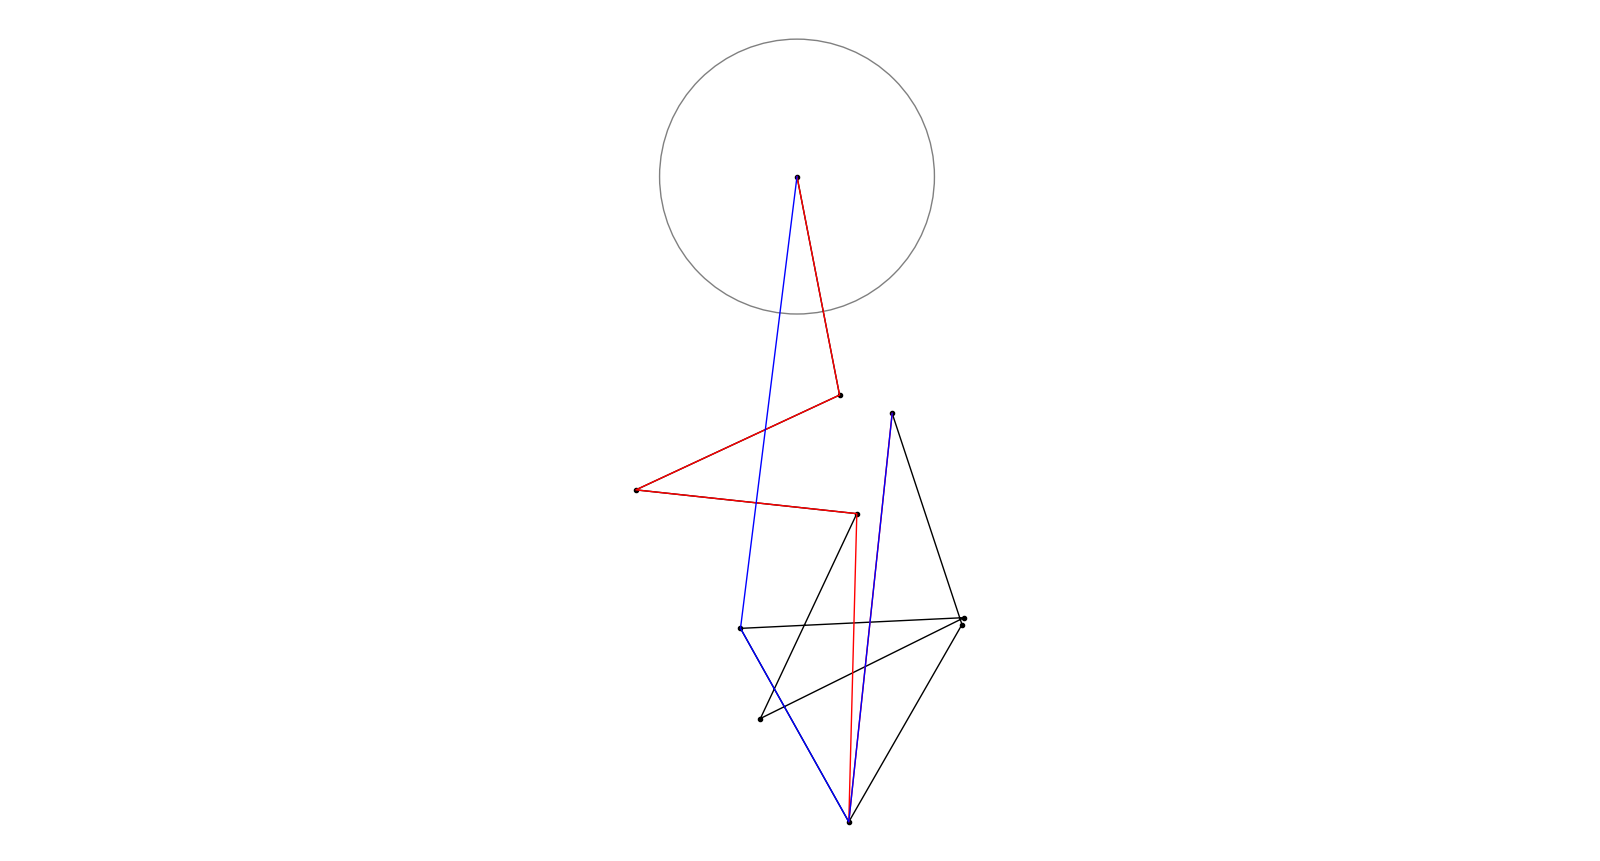
\includegraphics[scale=1, width=0.9\linewidth]{./figures/gii_diff_2.png}
	\caption{A negative polyline with 10 points. The difference between the heuristic and global simplification is 2. The last blue line segment is shared by both simplifications. The circle around \(P(0)\) has radius \(\varepsilon\).}
  \label{fig:gii_diff_2}
\end{figure}

We want to mention that we were not able to construct such an example ourselves. This example was found during testing on random polylines. We extracted the part that caused the difference into this example. Actually constructing polylines where the simplifications differ is non-trivial as negative mappings mostly arise in unintuitive substructures and to obtain a polyline with differing simplifications it is better to have multiple negative mappings.

\subsection{Conclusion}

This algorithm scheme generalizes \citeauthor{global_curve_simplification}'s algorithm and the \citeauthor{on_optimal_polyline_simplification_using_the_hausdorff_and_frechet_distance} algorithm but also the \citeauthor{computational_geometric_methods_for_polygonal_approximations_of_a_curve} algorithm. However, this approach is more complex than local simplification algorithms, and slower.

We have not shown any guarantees on our heuristic but it can easily be shown that is optimal on \cref{fig:local-global-bigdiff,fig:local-global-mostdiff} since those polylines are \(\varepsilon\)-proceeding. Thus, our heuristic is reasonable on some polylines where local simplifications suffer massively.

In their comprehensive study on global types of simplification, \citeauthor{global_curve_simplification} state ``what makes the problem difficult it is not well understood". We think our adaptation of the \citeauthor{computational_geometric_methods_for_polygonal_approximations_of_a_curve} algorithm to the global setting and the resulting heuristic make a convincing point that a negative mappings and the resulting need to mainting large structures is a major difficulty.

We conclude with further research questions regarding the global shortcut graph and our heuristic.

\begin{itemize}
	\item	How much can the heuristic differ from the optimum?

	We gave an example where it differed by 2 on a polyline of length 10. By replicating it with enough distance (similarly to \cref{fig:local-global-bigdiff}) we can create polylines with an arbitrary difference. However, this process can only create polylines where the difference is within a factor of \(1.5\). We do not know if the heuristic can be arbitrarily bad (like local simplifications) or whether an approximation guarantee can be established. We think that it can be arbitrarily bad by creating polylines with many negative mappings which reduce the intervals and thus disqualify many mappings which could be used for a global simplification but we have no construction to back this hypothesis.

	\item Which are strategies are there for the intervals and mappings?

	Our strategy is simple but comes with no guarantees as far as we know. More sophisticated update rules may allow for better simplifications while preserving the cubic time worst case and quadratic worst case space consumption.

	\item Under which conditions is a polyline positive or neutral?

	We have given some basic properties. However, our conditions are either trivial or are only useful as a certificate that the found heuristic is optimal. They are rather abstract which makes it hard to reason whether they are likely to apply to any class of polylines.

	\item Can the heuristic be implemented in (near-)quadratic runtime?

	For sufficiently nice polylines, the algorithm can achieve quadratic runtime. For this, there should be only few mappings and intervals, and the cell reachability to compute the mappings should use early exits as often as possible. 

	Our heuristic is structurally closer to the algorithm by \citeauthor{computational_geometric_methods_for_polygonal_approximations_of_a_curve} which has already been optimized to achieve that runtime (e.g. \cite{polyline_simplification_under_the_local_frechet_distance_has_almost_quadratic_runtime_in_2d_storandtetal}). It is still more complex than the local case as we do not only track one vertex but a list of intervals for each vertex. Some concept can be adapted, for example, \citeauthor{polyline_simplification_under_the_local_frechet_distance_has_almost_quadratic_runtime_in_2d_storandtetal} use wedges based on the unit circle around points to narrow down shortcuts. These can be adapted into the global setting by widening the wedges to all points on the respective subpolylines. 
\end{itemize}








